\documentclass{tudelft-report}


% 1)Translates MATLAB code:
\usepackage[framed,numbered,autolinebreaks,useliterate]{mcode}
% enclose the MATLAB code by using begin/end{lstlisting}

% 2)Multiple figures on one page
\usepackage{float}
\usepackage[caption = false]{subfig}

\begin{document}

%% Use Roman numerals for the page numbers of the title pages and table of
%% contents.
\frontmatter

\title[The analysis of data concerning the health of renal transplant patients]{Renal Transplant \\Health Analysis}
\author{Group C}
\affiliation{Faculty Electrical Engineering Mathematics and Computer Science}

\coverimage{cover.jpg}
\makecover[backboxheight = 4.3in]


%% Include an optional title page.
\begin{titlepage}

\begin{center}

%% Insert the TU Delft logo at the bottom of the page.
\begin{tikzpicture}[remember picture,overlay]
    \node at (current page.south)[anchor=south,inner sep=0pt]{
        
\includegraphics{cover/logo}
    };
\end{tikzpicture}

%% Extra whitespace at the top.
\vspace*{2\bigskipamount}

%% Print the title in cyan.
{\makeatletter
\titlestyle\color{tudelft-cyan}\Huge\@title
\makeatother}

%% Print the optional subtitle in black.
{\makeatletter
\ifx\@subtitle\undefined\else
    \bigskip
    \titlefont\titleshape\LARGE\@subtitle
\fi
\makeatother}

\bigskip
\bigskip

by
%door

\bigskip
\bigskip

%% Print the name of the author.
{\bfseries Group C} \\
Louis Gosschalk, Boudewijn van Groos, Jens Langerak, Chris Langhout \& Paul van Wijk \\
lgosschalk (4214528), bvangroos (4229843), jlangerak (4317327), clanghout (4281705), pvanwijk (4285034)

\vfill

in partial fulfillment of the requirements for the course of
%in overeenstemming met de vereisten voor het verkrijgen van de graad van

\bigskip
\bigskip

{\bfseries Context Project}

in Computer Science

\bigskip
\bigskip

at the Delft University of Technology,
%aan de Technische Universiteit Delft,

to be presented publicly on Friday June  26th, 2015.
%in het openbaar de verdedigen op dinsdag 1 januari om 10:00 uur.

\vfill

\begin{tabular}{ll}
%% Add additional information here, per faculty requirements, e.g
%    Student number: & 1234567 \\
%    Project duration: & \multicolumn{2}{l}{March 1, 2012 -- January 1, 2013} \\
    Project Coordinator: & Prof.\ Dr.\ A.\ Hanjalic\\
    	& Dr.\ A.\ Bacchelli\\
    Context Coordinator:
        & Dr.\ ir.\ W.\ P.\ Brinkman \\
    Software Engineering TA: & T.\ M.\ Hegeman
\end{tabular}

%% Only include the following lines if confidentiality is applicable.
\bigskip
\bigskip

\bigskip
\bigskip
An electronic version of this report is available at \url{https://github.com/clanghout/Health-Informatics-3/}.
%Een elektronische versie van dit verslag is beschikbaar op \url{http://repository.tudelft.nl/}.

\end{center}

\end{titlepage}



\chapter*{Abstract}
\setheader{Abstract}

There is a problem. A lot of patients of the ADMIRE project have to be analyzed but there is no analysis software simple enough to do this easily. So what do you do when you want to do something which should not require a lot of effort but no software exists to easily achieve this? Exactly, you build software for it.

To build this software we worked according to the SCRUM method and weekly presented a high fidelity prototype. This resulted in a software which, according to previous meetings, has grown to be accurately satisfying the needs of the customer. % lol quest giver

But why do we even care about these analyses? We care because these analysis might help us understand the patients better and thus might make it possible to improve the system and help the patients better with better advice, for example.

At the end of this project our conclusion is that we successfully understood and solved the problem through our implementation.

% abstract beschrijving zie http://users.ece.cmu.edu/~koopman/essays/abstract.html

\tableofcontents

%% Use Arabic numerals for the page numbers of the chapters.
\mainmatter

\chapter{Introduction} %MAX 1 PAGE

What have we done this project? How did we achieve to get where we are? In this report we will show you how, what, and why we have done what we have done.

We will start with a software overview, which will show the functionalities which have been implemented. A reflection on the software engineering will follow this, to explain how we went to work, what code requirements our group had set, how we handled feedback and more. To fully explain and describe the functionalities of the software, a feature description comes after the reflection, where all functionality aspects will come to discussion. After explaining the features a description will be given about how we managed to design and create our software to meet requirements which have been taught to us in the interaction design course. This will be followed by a product evaluation chapter to discuss the product in its entirety and last but not least we will give you an outlook on the future of our system. 
\chapter{Software Overview} %MAX 1 PAGE

Introduction to software overview. (what has been made, all must haves implemented, etc). 1 PAGE

\section{Must Have}
Describe all must haves that have been implemented.

\section{Should Have}
Describe the should haves which have been implemented.

\section{Additional Functionalities}
Describer any additional functionalities we have implemented (could \& would haves)
\chapter{Engineering Reflection} %MAX 1 PAGE

Introduce the chapter, explain what will be descibed. 2 PAGES

\section{GitHub Pulls}
It was not allowed to push changes directly to the master. When a person wanted to merge a change into the master he had to open a pull request. The pull request had to be approved by at least two team members before it could be merged with the master. The code for the pull request should contain comments and javadoc. Furthermore it should be tested and the code should have a good quality. And at last, the tools we use to evaluate the quality of the code, must say that the code was good. We look very critical to pull request. So often the one who had requested the pull requested had to improve some parts of his code. This led to good code quality. However most comments were related to code style and not directly to the implementation of the code.
The size of the pull requests varies a lot. In the beginning of the project they were very large. But since they were large, reviewing was difficult. And since they were large it was not possible to do the review quick, so people postponed the reviews. Therefore we tried to create smaller pull requests. This result of this was that pull requests were handled quicker and that we could review them better. However there were still some very large pull requests.
The time that a pull request was open varies a lot. Small reviews were most of the time handled within an hour. However large pull request stayed sometimes open for a very long time. For large pull request it could take sometimes days before it was reviewed and corrected again. So therefore we tried to keep the pull request small. The reviewing of the code, led to good code quality. 
\section{Code Quality}
Talk about the way we maintained quality in the code

\section{SIG Feedback}
Talk about how we made changes after SIG feedback 
\chapter{Feature Description}
%MAX 2 PAGES
Our program offers a variety in features. In this chapter these features are described.
\section{Import}
To specify the data used in the data model we use an XML file. Using a file to specify the data makes our program generic and easy to use since the same XML file can be used more than one time. \\
In the XML file all the needed information of a file is found. The path to the file is specified as well as the delimiter used. For each column a data type is specified. 
\subsection{XML wizard}
\begin{figure}[h!]
\centering
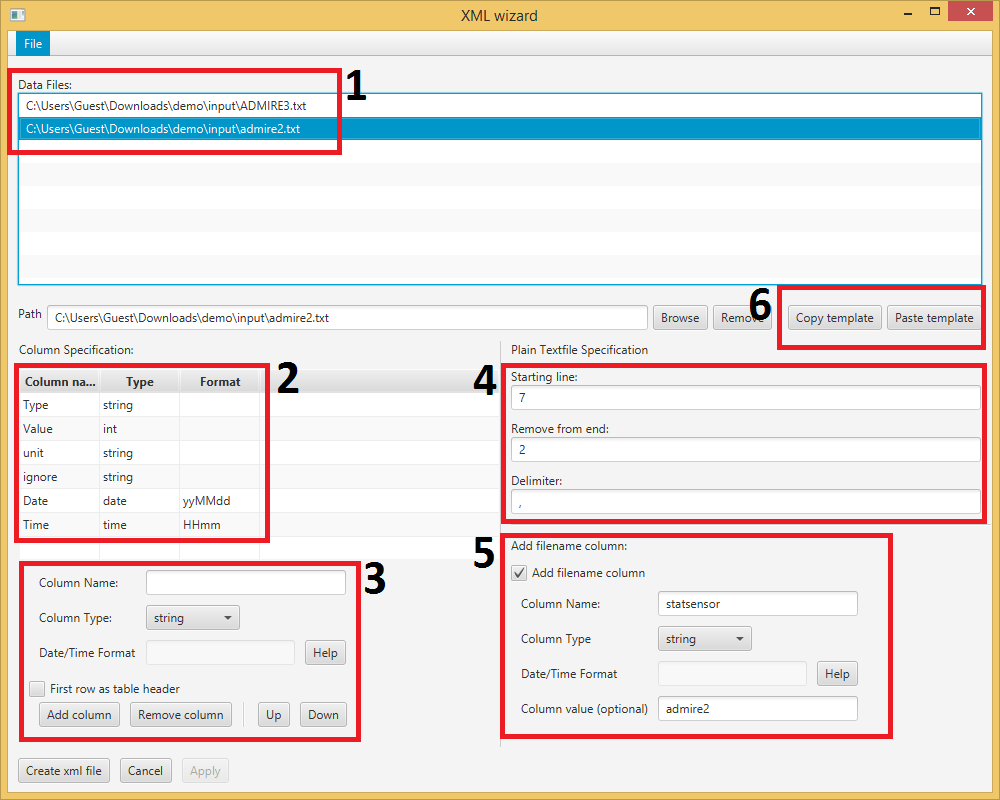
\includegraphics[width=300px]{chapters/image-featureDescription/xmlwizard-highlight.png}
\caption{The XML Wizard}
\end{figure}
To make it easier to make an XML file for our program, we created an XML wizard. In this wizard multiple files can be selected for the data [1]. Then per file, columns can be added with the appropriate type and (if needed) format [2, 3]. An option exists to use the first row as the column names. When this option is selected, no name needs to be specified for the columns in the wizard. The lines to skip at the start and the end of the file can be specified [4] and an option is available to add an extra column to the data containing the file-name or text specified by the user [5]. When all the settings are set, this info can be copied and then pasted for a similar file [6]. As in the example, multiple StatSensor files are loaded and use the same settings. 
\section{Analysis}
To analyse the data, the user has to switch to the 'analysis' tab. In this tab a text area is present where the user can add code in the program exclusive "SUGAR" language. When a script already exists, this file can simply be loaded into the program. This script can be changed and executed to affect the data. After changes are made, the script can be saved to file again. 
\subsection{The C's}
Multiple different analyses exist to execute on data. Following the terminology of EDA we implemented 6 out of the Eight C's of the generic ESDA process\cite{analysis}:
\subsubsection{Constraint}
A constraint can be used to select specific values from a column. Numbers can be compared to constants or other columns. Constraints can also be combined with AND, OR and NOT operations. On date values, the extra constraints "before" and "after" are available. 
\subsubsection{Computation}
Number values can be added, divided, multiplied and subtracted. The modulo operation is available, as well as the square root and the power function. Date values can be added or subtracted and the relative difference can be computed. Separate date and time can be combined to one DateTime value, also the opposite; DateTime values can be split up to either date or time value. All the computations can also be used in the constraints in combination with column values or constants.
\subsubsection{Comparison}
To determine a relation between events, the lag sequential comparison is available. The lag sequential analysis will return a table chronologically sorted on the events.
%lag sequential
\subsubsection{Code}
Codes can be added to rows when a value of that row satisfies a constraint. A single row can contain zero or more codes. When a row contains a code, it can be selected via a specific constraint that selects only that code. 
\subsubsection{Chunking}
Chunks can be created with the group by function. A group by function can be applied on a column or on a constraint combined with a column. This creates a new table with the first column the value of the group, the following columns are created after the functions given by the user, applied to that column.
\subsubsection{Connections}
To connect two or more tables, a join function is available. Tables can be joined in multiple ways. The full join is available as well as a left, right and simple join.
\subsection{Additional Analyses}
Apart from the implemented C's, more functions can be used in the program.  
\subsubsection{Union}
Two tables can be unified with the union command. This creates a new table with only the rows that have the same values in both tables. Codes of the rows of the two tables are not taken into account when comparing, but when two rows are the same the codes of both rows are combined in the new table.
\subsubsection{Difference}
The opposite of the union is also possible, the difference operation. Two tables are subtracted and only unique rows are added to the resulting table.
\section{Visualize}
No analysis is finished without visualizing the data. A visualization shows the data in an easy and fast interpretable way. In the visualization tab of the program buttons can be pressed to show a pop-up where the data for that visualization can be specified. After a visualization is made, the image can be saved as PNG file.
\subsection{Box-plot}
A single box-plot can be created of one column with the FloatValue or IntValue type. This happens in the graph pop-up where first a table is selected and then the column can be selected. The support of creating multiple box-plots at once is not implemented but it is possible to save box-plots one by one.
\subsection{Bar-chart}
A bar-chart can also be made via the graph pop-up. For the bar chart's axes, two columns must be selected. An example for the x-axis could be the names of created chunks since these are unique. For the y-axis a column with NumberValues must be picked. 
\subsection{State-Transition-Matrix}
The state-transition-matrix has its own pop-up menu. When no codes are present, the pop-up shows an error message and no matrix can be created because codes represent the states in the matrix. When a table is selected, a column can be selected to define the order of the table. Then the user can select the codes to add in the state-transition-matrix. When the create button is pressed, a matrix is created with the amount of transitions between the selected states as values.

\chapter{Interaction Design} %MAX 2 PAGES
In this chapter we will describe the interaction design test we have done with the user. First we will describe the persona of a typical user of the tool and next we will tell how the test. Furthermore we will draw the conclusions from the test.

\section{Methods}
We put the user behind the computer and asked him to perform tasks. We first wanted him to read in files and then perform analyses. If the user can not figure out how to do something, we gave some hints to help him along the way. The more complicated analyses were pre-written so that the user only has to modify the existing analysis to make it work. We did this because the language we use has a high learning curve and we did not have a lot of time at the test to make the user learn the complete language.

\section{Expectation}
In this section we will describe what we expected how the test would go. We expected that the test could be a bit too difficult. This is because the the language we use is not that easy to understand at the first time using it. We provided the users with some example scripts of the language to make this process easier.
We expected that the graphical user interface would be easier to understand.

\section{General Persona}
In this section we will describe John Doe who is an abstraction of our typical user.\\
John is an analyst and he uses analysis tools on a regular basis. His analyses are performed on data that is collected during research. He has a specific goal in mind and he wants to get to an answer to a specific question about the data. John also has minimal experience in programming, but is familiar with scripts from other analysis tools and is eager to learn a new scripting language.

\section{Evaluations}
Every Friday the team had a meeting with the client to show progress and get feedback on the demo. To show our progress to the client we used the high fidelity prototyping principle.
\subsection{Usability evaluation}
To test the usability and functionality of the program, tests are done with our client Miss Wang. A meeting was arranged where the program was used by the client and the functionalities of the program were shown. For the example questions that the client wants to answer pre-made scripts were executed and feedback was given on the overall process.\\
Little things were changed as a result of the meeting, for example the save button was moved because right below the import button did not make sense. We also discovered during this meeting that the visualizations did not work anymore due to changes in parts the visualizations are dependant on. Overall the client was positive about the product since most of the analyses could be executed.
\subsection{Additional test results}
Other tests were done with fellow students. The detailed results are found in appendix \ref{ch:results}.\\
Generally the tests resulted that our language is quite difficult to understand, which was already predicted. The user interface was generally clear and only little remarks were made on positioning of buttons. With the provided examples of analysis scripts the testers could reproduce a similar analysis with reasonable effort. Most of the time it was clear which part of the interface belonged to which feature with little exception in the visualization selection. The general impression of the program was good, the interface is clear analysis functionality is good.
\chapter{Product Evaluation} %MAX 2 PAGES

\section{Product}
Even though our product has many features, it can be reduced to five simple modules:
\begin{itemize}
	\item The Data Importation Module
	\item The Data Viewing Module
	\item The Data Exportation Module
	\item The Analysis Module
	\item The Visualization Module
\end{itemize}
These are the same modules that'd been mentioned in the first context specific lecture, so in general we managed to implement the most required features. For our features we focused mostly on the must haves. These were roughly specified in the first lectures and after a couple of weeks we got the actual product requirements.

We'd hoped to finish the must haves early and perhaps tackle a couple of could haves. However due to some issues we encountered we had to adjust our planning to finish all the must haves. This meant that some features we were hoping to get in didn't make the cut.

Overall we must say that it is really hard to anticipate exactly how the final product will turn out. You have an idea of which features you should provide, but the way all those features work together is something else entirely. In the end we're satisfied with the result and how everything turned out. We missed the time to really polish it up and get all the bugs out of there, but it is a program which does what it is supposed to and it can do a whole lot more.

\section{Modules}
In this section we'll discuss the precise operation of the various modules.

\subsection{Data Importation}
The data importation module consists of two parts: the data reading part and the data describing part. The data reading part takes an XML file which can be generated using the data describing part. We've noticed the describing process isn't completely intuitive and it is something we should have spend more time on. That being said, the process in itself is rather complex and a UI can only get you so far.

\subsection{Data Viewing}
The data viewing module is rather simple. You have a list of the left of the various tables present in the program and a table on the right showing the contents of the table. There is also a button to save a table which opens a wizard, more on this in the next section. This module is rather simple and we're satisfied with its simplicity.

\subsection{Data Exportation}
This module consists of a dialog which can be used to save a table to a file. It's got a couple of simple options to select how exactly the file is to be saved and it's all very user-friendly.

\subsection{Analysis}
The analysis module consists of a textbox and a couple of buttons to run, save and load scripts. This is by far the largest module as the entire point of our program was performing those analyses. We support a great number of analyses and some other processes which can do some rather complicated stuff with the input data. We wish we'd implemented a couple more analyses, but there was only so much we could do in the given time. In the end we're content with the rather complicated, yet subtle workings of our language. We do realize that the complex workings of our language present the user with a bit of a challenge to learn our language.

\subsection{Visualization}
In the visualization module we support generating a box plot, frequency graph and state transition matrix. All of this is done through a simple dialog, which is simple and easily understandable. We do think that a little more time could have polished it up a bit and removed a couple of bugs. However the graphs created are pretty and useful. Also we don't think that the visualization is the core part of our program, there exist other better tools to do such things.

\section{Failure Analysis}
In this section we'll discuss the various issues that are still present in the program.

One of the major issues we encountered in the realisation process was that Java generics aren't available in runtime. This is something we encountered along the way and didn't anticipate beforehand. Currently it means that we're not able to do type checking in our language. So multiplying a date by a boolean is okay for the parser and it will throw a non descriptive runtime exception. In the future I think it is something we'll take into account when dealing with generics.

One of the other major issues is that our program isn't very user friendly. This isn't a major concern as the program is very specialistic and the main target audience is very limited. However it is something we should have paid more attention to. 

Another issue is one of performance. The data that is entered in our program is quite large and it  hasn't been optimized one bit. This means the user has to wait a while for the larger analyses. However it is perfectly possible to reduce the data by performing a simple analysis. This should speed things up for the user.

Last of all there is a bug in the visualization module: an error message doesn't go away when it should, this could have been solved by testing more thoroughly.
\chapter{Outlook}
Describe possible improvements for the future and strategy to implement those, should the software be used.


%% Use letters for the chapter numbers of the appendices.
\appendix

\begin{table}[h]
\begin{tabular}{llll}
User Story & Task & Task assigned to & Estimated effort per task \\
User story 1 description & 
\begin{itemize}
\item Task description 1
\item Task description 2
\item Task description 3
\end{itemize} & 1 & 1 \\

User story 1 description & 1 & 1 & 1 \\

User story 1 description & 1 & 1 & 1
\end{tabular}
\end{table}
\chapter{Sprint Reflections}


\bibliography{report}

\end{document}

